% !TEX TS-program = XeLaTeX
% use the following command: 
% all document files must be coded in UTF-8
\documentclass[spanish]{textolivre}
% See more information on the repository: https://github.com/leolca/textolivre

% Metadata
\begin{filecontents*}[overwrite]{article.xmpdata}
    \Title{Aplicaciones que emplean y recomendaciones que entregan docentes universitarios para la autorregulación del aprendizaje en contexto de la pandemia por COVID-19}
    \Author{Valeria Aylín Infante-Villagrán \sep Bianca Maria Pia Dapelo Pellerano \sep Rubia Cobo-Rendon \sep Yaranay López-Angulo \sep Bertha Escobar Alaniz \sep Christian Beyle}
    \Language{es}
    \Keywords{Aplicaciones digitales \sep Enseñanza virtual \sep Docencia  universitaria \sep COVID-19}
    \Journaltitle{Texto Livre}
    \Journalnumber{1983-3652}
    \Volume{14}
    \Issue{3}
    \Firstpage{1}
    \Lastpage{23}
    \Doi{10.35699/1983-3652.2021.33027}

    \setRGBcolorprofile{sRGB_IEC61966-2-1_black_scaled.icc}
            {sRGB_IEC61966-2-1_black_scaled}
            {sRGB IEC61966 v2.1 with black scaling}
            {http://www.color.org}
\end{filecontents*}

\journalname{Texto Livre}
\thevolume{14}
\thenumber{3}
\theyear{2021}
\receiveddate{\DTMdisplaydate{2021}{4}{8}{-1}} % YYYY MM DD
\accepteddate{\DTMdisplaydate{2021}{5}{31}{-1}}
\publisheddate{\DTMdisplaydate{2021}{8}{30}{-1}}
% Corresponding author
\corrauthor{Bianca Maria Pia Dapelo Pellerano}
% DOI
\articledoi{10.35699/1983-3652.2021.33027}
%\articleid{NNNN} % if the article ID is not the last 5 numbers of its DOI, provide it using \articleid{} commmand
% list of available sesscions in the journal: articles, dossier, reports, essays, reviews, interviews, editorial
\articlesessionname{articles}
% Abbreviated author list for the running footer
\runningauthor{Infante-Villagrán et al.}
\sectioneditorname{Daniervelin Pereira}
\layouteditorname{Anna Izabella M. Pereira}

\title{Aplicaciones que emplean y recomendaciones que entregan docentes universitarios para la autorregulación del aprendizaje en contexto de la pandemia por COVID-19}
\othertitle{Aplicativos usados e recomendações dadas por professores universitários para a autorregulação da aprendizagem no contexto da pandemia de COVID-19}
\othertitle{Applications used and recommendations provided by university professors for self-regulation of learning in the context of COVID-19 pandemic}
% if there is a third language title, add here:
%\othertitle{Artikelvorlage zur Einreichung beim Texto Livre Journal}

\author[1]{Valeria Aylín Infante-Villagrán~\orcid{0000-0002-1593-0468}~\thanks{Email: \url{valeria.a.infante.v@gmail.com}}}
\author[2]{Bianca Maria Pia Dapelo Pellerano~\orcid{0000-0001-5357-3900}~\thanks{Email: \url{bdapelo@uvm.cl}}}
\author[3]{Rubia Cobo-Rendon~\orcid{0000-0002-3350-071X}~\thanks{Email: \url{rubiacobo@udec.cl}}}
\author[1,4]{Yaranay López-Angulo~\orcid{0000-0002-3331-6875}~\thanks{Email: \url{yara13190@gmail.com}}}
\author[5]{Bertha Escobar-Alaniz~\orcid{0000-0001-5768-1845}~\thanks{Email: \url{bescobar@uct.cl}}}
\author[6]{Christian Beyle~\orcid{0000-0003-2526-3141}~\thanks{Email: \url{cbeyle@gmail.com}}}

\affil[1]{Universidad de Concepción, Facultad de Ciencias Sociales, Departamento de Psicología, Doctorado en Psicología, Concepción, Región del Bío-Bío, Chile.}
\affil[2]{Universidad Viña del Mar, Escuela de Ciencias Jurídicas y Sociales. Viña del Mar, Región de Valparaíso, Chile.}
\affil[3]{Universidad de Concepción, Laboratorio de investigación e innovación educativa IDEClab, Dirección de Docencia, Concepción, Región del Bio-Bio, Chile.}
\affil[4]{Universidad Santo Tomás, Facultad de Ciencias Sociales y Comunicaciones, Escuela de Psicología, Concepción, Chile.}
\affil[5]{Universidad Católica de Temuco, Facultad de Ciencias de la Salud, Departamento de Psicología, Temuco, Región de La Araucanía, Chile.}
\affil[6]{Universidad Católica de Temuco, Departamento de Psicología, Temuco, Región de La Araucanía, Chile.}


\addbibresource{article.bib}
% use biber instead of bibtex
% $ biber tl-article-template

% set language of the article
\setdefaultlanguage{spanish}
\setotherlanguage{portuguese}
\setotherlanguage{english}

% for spanish, use:
%\setdefaultlanguage{spanish}
\gappto\captionsspanish{\renewcommand{\tablename}{Tabla}} % use 'Tabla' instead of 'Cuadro'
\AfterEndPreamble{\crefname{table}{tabla}{tablas}\Crefname{table}{Tabla}{Tablas}}

% for languages that use special fonts, you must provide the typeface that will be used
% \setotherlanguage{arabic}
% \newfontfamily\arabicfont[Script=Arabic]{Amiri}
% \newfontfamily\arabicfontsf[Script=Arabic]{Amiri}
% \newfontfamily\arabicfonttt[Script=Arabic]{Amiri}
%
% in the article, to add arabic text use: \textlang{arabic}{ ... }

% for russian text we also need to define fonts with support for Cyrillic script
% \usepackage{fontspec}
% \setotherlanguage{russian}
% \newfontfamily\cyrillicfont{Times New Roman}
% \newfontfamily\cyrillicfontsf{Times New Roman}[Script=Cyrillic]
% \newfontfamily\cyrillicfonttt{Times New Roman}[Script=Cyrillic]
%
% in the text use \begin{russian} ... \end{russian}

% to use emoticons in your manuscript
% https://stackoverflow.com/questions/190145/how-to-insert-emoticons-in-latex/57076064
% using font Symbola, which has full support
% the font may be downloaded at:
% https://dn-works.com/ufas/
% add to preamble:
% \newfontfamily\Symbola{Symbola}
% in the text use:
% {\Symbola }

% reference itens in a descriptive list using their labels instead of numbers
% insert the code below in the preambule:
\makeatletter
\let\orgdescriptionlabel\descriptionlabel
\renewcommand*{\descriptionlabel}[1]{%
  \let\orglabel\label
  \let\label\@gobble
  \phantomsection
  \edef\@currentlabel{#1\unskip}%
  \let\label\orglabel
  \orgdescriptionlabel{#1}%
}
\makeatother
%
% in your document, use as illustraded here:
%\begin{description}
%  \item[first\label{itm1}] this is only an example;
%  % ...  add more items
%\end{description}
 

% custom epigraph - BEGIN 
%%% https://tex.stackexchange.com/questions/193178/specific-epigraph-style
\usepackage{epigraph}
\renewcommand\textflush{flushright}
\makeatletter
\newlength\epitextskip
\pretocmd{\@epitext}{\em}{}{}
\apptocmd{\@epitext}{\em}{}{}
\patchcmd{\epigraph}{\@epitext{#1}\\}{\@epitext{#1}\\[\epitextskip]}{}{}
\makeatother
\setlength\epigraphrule{0pt}
\setlength\epitextskip{0.5ex}
\setlength\epigraphwidth{.7\textwidth}
% custom epigraph - END


% if you use multirows in a table, include the multirow package
\usepackage{multirow}

% add line numbers for submission
%\usepackage{lineno}
%\linenumbers

\begin{document}
\maketitle

\begin{polyabstract}
\begin{abstract}
El uso estratégico de las aplicaciones digitales en educación superior adquiere especial relevancia en tiempos de pandemia por COVID-19. Se presenta un estudio exploratorio en el cual se indaga en el uso de  aplicaciones digitales y las que recomiendan  docentes universitarios para la autorregulación del aprendizaje en contexto de  enseñanza virtual, por COVID-19. La metodología fue de carácter cualitativa, con un enfoque fenomenográfico, basado en tres grupos focales, con una muestra intencional de 17 docentes. Los datos fueron analizados a través de la técnica de Análisis de Contenido. Se identifican 27 aplicaciones digitales pertinentes para facilitar la autorregulación del aprendizaje, las cuales fueron agrupadas según el modelo cíclico de Zimmerman, 16 fueron útiles para la fase de preparación, 19 para la fase de ejecución, 11 para la fase de autorreflexión y 8 para las tres fases del modelo. WhatsApp y Google Calendar son las aplicaciones más recomendadas para los procesos de autorregulación, específicamente para la disposición del aprendizaje. La convergencia de conocimiento sobre autorregulación del aprendizaje y competencias TIC emergen como un desafío compartido para promover el uso estratégico de las aplicaciones digitales y  favorecer aprendizajes inclusivos y de calidad en la universidad, en contexto de pandemia por COVID-19. 

\keywords{Aplicaciones digitales \sep Enseñanza virtual \sep Docencia  universitaria \sep COVID-19}
\end{abstract}

\begin{portuguese}
\begin{abstract}
O uso estratégico de aplicativos digitais no ensino superior adquire especial relevância em tempos de pandemia de COVID-19. É apresentado um estudo exploratório no qual são identificadas as aplicações digitais que os professores universitários chilenos utilizam e aquelas que eles recomendam para a autorregulação da aprendizagem no contexto do ensino virtual, devido à pandemia de COVID-19. A metodologia foi de natureza qualitativa, com abordagem fenomenográfica, a partir de três grupos focais, com amostra intencional de 17 professores. Os dados foram analisados por meio da técnica de Análise de Conteúdo. 27 aplicativos digitais relevantes são identificados para facilitar a autorregulação da aprendizagem, 16 úteis para a fase de preparação, 19 para a fase de execução, 11 para a fase de autorreflexão e 8 para as três fases do modelo cíclico de Zimmerman. WhatsApp e Google Calendar são os aplicativos mais recomendados para processos de autorregulação, especificamente para a disposição do aprendizado. A convergência de conhecimentos sobre a autorregulação da aprendizagem e competências em TIC surgem como um desafio partilhado para promover uma utilização estratégica das aplicações digitais e favorecer a aprendizagem inclusiva e de qualidade na universidade, no contexto da pandemia de COVID-19.

\keywords{Aplicações digitais \sep Ensino virtual \sep Ensino universitário \sep COVID-19}
\end{abstract}
\end{portuguese}

\begin{english}
\begin{abstract}
The strategic use of digital applications in higher education has been given special relevance in times of COVID-19 pandemic. This exploratory study inquires which digital applications are used and recommended by Chilean higher education lecturers in order to promote self-regulated learning on the virtual education context. The methodology was qualitative, with a phenomenographic approach, based on three focus groups, with an intentional sample of 17 lecturers. The data was analyzed through Content Analysis technique. 27 relevant digital applications were identified to facilitate self-regulation of learning, 16 useful for the preparation phase, 19 for the execution phase, 11 for the self-reflection phase, and 8 for the three phases of the Zimmerman cyclical model. WhatsApp and Google Calendar are the most recommended applications for self-regulation processes, specifically for the disposition of learning. The reciprocal influence of knowledge on self-regulation of learning and ICT skills emerges as a shared challenge to promote a strategic use of digital applications and to foster inclusive and quality learning in the university, in the context of emergency online education.

\keywords{Digital applications \sep Virtual teaching \sep University teaching \sep COVID-19}
\end{abstract}
\end{english}

% if there is another abstract, insert it here using the same scheme
\end{polyabstract}


\section{Introducción}\label{sec-intro}
El contexto de la pandemia por COVID-19 ha transformado abruptamente la educación en todo el mundo, obligando a las instituciones educativas a transitar desde una modalidad de enseñanza-aprendizaje presencial a una virtual de emergencia en pocas semanas, generando cambios en los modos de interacción social \cite[p. 59]{gazzo2020}, situación para la cual, no todo el profesorado y actores educativos estaban preparados \cite[p. 5]{bancointeramericano2020}. Esta transformación repentina en la modalidad de enseñanza ha ocasionado una merma en la calidad de los aprendizajes y un incremento en la deserción en todos los niveles educativos \cite[p. 37]{instituto_internacional_para_la_educacion_superior_en_america_latina_y_el_caribe_covid-19_2020} y al mismo tiempo, ha levantado múltiples desafíos, entre los que se encuentra la necesidad de desarrollar habilidades de autorregulación del aprendizaje por parte de los  estudiantes, por su diversidad en conocimientos, preparación o motivación para regular y dirigir su propio aprendizaje \cite[p. 78]{marcelo2019}.

La autorregulación del aprendizaje es un proceso activo, en el cual los  estudiantes fijan objetivos, supervisan y regulan sus estados cognitivos, motivacionales y comportamentales para lograr el aprendizaje \cite[p. 140]{perez2013}. Así, puede concebirse como un constructo multidimensional, que integra dimensiones motivacionales, metacognitivas y emocionales \cite[p. 125]{gonulkurt2016}, donde un factor clave es el ambiente de aprendizaje, lo que hace relevante la participación docente en su desarrollo \cite[p. 84]{artino2012}.

Según el modelo propuesto por \textcite[p. 142]{zimmerman2013} el uso de estrategias para la autorregulación del aprendizaje comprende tres fases cíclicas: 1) fase de preparación, compuesta por dos procesos: análisis de la tarea y las creencias de auto-motivación. En el análisis de la tarea los  estudiantes se fijan metas e idean un plan para alcanzarlas. Respecto de las creencias de auto-motivación, los  estudiantes evalúan el valor que tienen las tareas y regulan sus esfuerzos y motivaciones de acuerdo a sus creencias de autoeficacia; 2) fase de ejecución, en la que toman protagonismo los procesos de autocontrol y auto-observación. En el primero, los  estudiantes gestionan estrategias para alcanzar sus metas, mientras que, en el segundo, llevan a cabo un monitoreo metacognitivo del propio rendimiento; y 3) fase de autorreflexión, en la que cobran relevancia los procesos cognitivos, emocionales y conductuales. Esta fase incluye aspectos relacionados con los auto-juicios y auto-reacciones.

En este sentido, una de las estrategias que ha sido ampliamente utilizada por el cuerpo docente en los últimos años para involucrar a los  estudiantes en su aprendizaje es el uso de tecnología, entre las que se destacan las aplicaciones digitales. Las aplicaciones digitales o App, son herramientas que pueden ser usadas en un servidor web o en sistemas operativos móviles como Android, iOS, Windows IPhone, entre otros. Las App basadas en la web se presentan en formato de recursos y herramientas que los  usuarios pueden utilizar por medio de un servidor web a través de internet desde un navegador. Mientras que las App nativas están diseñadas para ser utilizadas en dispositivos móviles y explotar las características de estos. También existe un tercer tipo de App denominadas híbridas, las cuales resultan de una combinación de App nativas y basadas en la web \cite[p. 12-13]{santiago_mobile_2015}.

Considerando que las generaciones de estudiantes actuales han nacido en una sociedad mediada por las App digitales y la tecnología digital, se han modificado los modos de organizar el aprendizaje y transmitir el conocimiento. Sin embargo, la educación remota de emergencia  debido a la pandemia por COVID-19 ha revelado por una parte, que no todo el profesorado es competente en los entornos digitales, especialmente los que vienen de una generación menos tecnológica \cite[p. 16-17]{cervantesgutierrez2020} y por otra, que los  estudiantes requieren mayor compromiso en este contexto, siendo “difícil prever los impactos que pueda tener el cambio de modalidad de enseñanza y aprendizaje a mediano y largo plazo” \cite[p. 22]{instituto_internacional_para_la_educacion_superior_en_america_latina_y_el_caribe_covid-19_2020}.

El uso de las plataformas o aulas virtuales construidas para el aprendizaje electrónico, permite al cuerpo docente contar con espacios donde crear y entregar contenido audiovisual a sus estudiantes, interactuar y monitorear su participación en los cursos \cite[p. 3]{ashrafi2020}. En tal sentido, las App educativas pueden constituir una oportunidad para la renovación metodológica en Educación Superior, resaltando el valor de la relación docente-estudiante en la promoción de interacciones que potencien procesos autorregulatorios \cite[p. 69]{zimmerman2002}. 

En el escenario de la Pandemia por COVID-19, diversas investigaciones han mostrado resultados sobre el uso de distintas App por docentes universitarios. Se ha identificado alta aceptabilidad y percepción positiva sobre el uso de la plataforma de Microsoft Teams para el desarrollo de sus cursos durante la pandemia \cite{zamora-antunano2021}. Se ha reportado el uso de otras  plataformas como WhatsApp, Zoom, Google Meets para el desarrollo de los procesos de enseñanza y aprendizaje \cite{almarzooq2020, budianto2021, akaloo2021, pramana2021} reportando en su mayoría, percepciones positivas sobre el uso de estos recursos para la enseñanza y comunicación con sus estudiantes. 

Por otro lado, se ha reportado una subutilización de los recursos virtuales y de los potenciales pedagógicos inexplorados de la plataforma Moodle \cite[p. 74]{valenzuela2013}, como su efectividad para fomentar la autorregulación del aprendizaje \cite[p. 495]{martinez-sarmiento2018}; y se ha señalado que las aplicaciones en contextos educativos, como foros virtuales \cite[p. 37]{castro2016}, blogs \cite[p. 182]{delgado2018}, redes sociales como WhatsApp \cite[p. 80]{weepiu2020}, entre otros, no aseguran el desarrollo de procesos de autorregulación por sí mismas, puesto que su potencial depende del modo en que el cuerpo docente diseñe las tareas académicas \cite[p. 17]{valencia2017} e intencionen las estrategias didácticas \cite[p. 80]{weepiu2020}, destacando el rol de la docencia en la motivación y participación \cite[p. 37]{castro2016}.

Así, en un entorno de enseñanza-aprendizaje virtual, resulta crucial el acompañamiento docente en el proceso autorregulatorio, siendo especialmente relevante en contexto de pandemia, dado el valor del apoyo social del profesorado \cite[p. 17]{lopezangulo2020}. La integración de tecnología, desde el diseño de los procesos de la clase, las dinámicas promotoras de un discurso regulador sobre la actividad cognitiva del estudiantado \cite[p. 8]{ninocarrasco2019}, la retroalimentación formativa y la generación de espacios para la autorreflexión \cite[p. 272]{valencia-serrano2020}, tienen un alto potencial para facilitar las fases del proceso de autorregulación del aprendizaje. Resulta menester que el cuerpo docente anticipe un conjunto de factores relacionados a la tarea, al estudiante y contexto que convergen en la situación didáctica y modulan la proyección de su efectividad, a la hora de generar oportunidades de autorregulación del aprendizaje \cite{castro2016, valencia2017}, de modo que la incorporación de tecnologías no resulte perjudicial para quienes se encuentran en situación de desventaja en educación virtual. En este sentido, las instituciones educativas deben encontrar la tecnología digital más apropiada para el contexto de sus actores, generando oportunidades de mejora en los procesos de enseñanza y aprendizaje \cite[p. 54]{instituto_internacional_para_la_educacion_superior_en_america_latina_y_el_caribe_covid-19_2020}.

Si bien se ha señalado que las App han incrementado en variedad y uso, son escasos los estudios que investigan su uso estratégico en el escenario de educación virtual, sobre todo para fomentar los procesos de autorregulación. Una revisión sistemática sobre estudios publicados entre 2006 y 2016, referentes a recursos para fomentar la autorregulación del aprendizaje en estudiantes de entornos digitales, evidencia una falta de herramientas para apoyar al estudiantado en esta modalidad \cite{wong2018}. Si bien la investigación actual presenta algunas propuestas, muy pocas alcanzan la etapa de implementación \cite[p. 1096]{perezalvarez2018}.

Es importante destacar que el estudiantado no acostumbra a hacer uso de las tecnologías digitales para apoyar su proceso de aprendizaje, más bien utilizan dichas tecnologías para compartir, buscar y recibir información \cite[p. 71]{marcelo2019}. Desprendiéndose de aquí la necesidad de preparar al cuerpo docente para el uso estratégico de la tecnología, que fomente el proceso de autorregulación del aprendizaje, en vista del relevante rol modelador que cumple el profesorado en el acompañamiento de dicho proceso \cite[p. 90]{diazmujica2017}, de esta manera el profesorado, teniendo el conocimiento suficiente podrían recomendar el uso de App para el fomento de la autorregulación del aprendizaje. Considerando esto surge la pregunta: ¿Qué aplicaciones digitales han utilizado docentes universitarios de Chile para promover la autorregulación del aprendizaje en contexto de enseñanza virtual por pandemia COVID-19?, y en este sentido, ¿qué aplicaciones digitales  han recomendado a estudiantes y docentes?

Para responder a esta pregunta el equipo de investigación desarrolla un estudio con diseño exploratorio secuencial de tipo mixto \cite{creswell2018}. En  este artículo, sólo se reporta la  primera fase, que recoge información cualitativa  acerca de la experiencia de docentes universitarios  en relación al empleo  de  aplicaciones digitales para el aprendizaje autorregulado y  aquellas  que  recomiendan para estos propósitos, en  contexto de enseñanza virtual por pandemia.

Así, en este trabajo se plantearon dos objetivos: (1) Explorar el empleo de App para la autorregulación del aprendizaje en contexto de enseñanza virtual por pandemia en un grupo de  docentes universitarios chilenos e (2) Identificar las recomendaciones que entrega el cuerpo docente universitario a estudiantes y docentes, para facilitar la autorregulación del aprendizaje en contexto de pandemia COVID-19.

\section{Método}
\subsection{Diseño}
Se utilizó un diseño fenomenográfico \cite[p. 189]{marton1981}. Dado el carácter exploratorio del estudio, cuyo problema se sitúa en el análisis del uso  estratégico de la tecnología en la  enseñanza universitaria virtual por COVID-19. Se empleó la metodología cualitativa que permite indagar la perspectiva docente respecto al empleo de aplicaciones digitales y  a su  recomendación, con el propósito de facilitar la autorregulación del aprendizaje en contexto de enseñanza virtual por pandemia.

\subsection{Participantes}
\subsubsection{Selección de la muestra de grupos.}
El presente estudio se realizó con una muestra integrada por 17 docentes universitarios, 12 mujeres y 5 hombres,  todos  con docencia virtual, en primer año de carreras de Ciencias de la Salud, Ciencias Sociales, Humanidades, Ciencias Básicas e Ingeniería, durante 2020, integrantes de 4 universidades, ubicadas en la zona centro sur de Chile, entidades asociadas al proyecto COVID-1012 “Desarrollo e implementación de procedimientos docentes para facilitar la disposición al aprendizaje en condiciones de distanciamiento físico por pandemia de COVID-19, en asignaturas de primer año universitario con mediano o alto riesgo de fracaso”. Se trató de una muestra intencional, no probabilística, de casos tipo \cite{hernandez2018} seleccionada a través de listados que aportaron los directivos del proyecto. El grupo de docentes participó voluntariamente, con consentimiento informado. El estudio contó con la aprobación del comité de ética de la Universidad de Concepción en el contexto del proyecto. 

\subsubsection{Características de los grupos.}
En coherencia con los propósitos del estudio se consideraron pertinentes dos criterios de inclusión que permitieran levantar una variedad de experiencias y opiniones. Estos fueron: (a) conocimientos en el fomento de autorregulación del aprendizaje adquiridos por medio de estudios o actualización en autorregulación en los últimos cinco años y /o (b) experiencia en el uso de tecnología para el fomento de autorregulación del aprendizaje de al menos de un año. El grupo de participantes potenciales, docentes con características del perfil, se ubicaron de los listados de profesionales disponibles en bases de datos del proyecto COVID-1012, fueron contactados por mail  e invitados a participar con diez días de antelación y una semana antes de su desarrollo para confirmar su interés por participar. Se procuró maximizar la similaridad de la muestra de participantes en cada grupo focal; en el primero participaron 7 docentes con conocimientos en el fomento de autorregulación del aprendizaje, en el segundo y tercero, se tuvo una concurrencia de 5 docentes con experiencia en uso de tecnología para el fomento de la autorregulación del aprendizaje en cada uno, ajustándose a lo sugerido por \textcite{krueger2006} respecto al número de participantes.

\subsection{Técnica para la obtención de información}
Se seleccionó la técnica de grupo focal, por su pertinencia para la exploración inicial de la problemática en estudio y por su ventaja de facilitar el acceso a información detallada en un periodo corto de tiempo \cite{johnson2008}, considerando que este reporte corresponde a la primera parte (cualitativa) de un estudio mixto, para el posterior desarrollo de una encuesta. Se ha señalado que “los grupos focales son básicamente grupos de discusión colectiva” \cite[p. 181]{mella2003}, constituyendo una herramienta valiosa por el aprendizaje que genera la discusión grupal en torno a las experiencias y opiniones de docentes, sobre una temática de interés compartida por  investigadores y participantes, permitiendo obtener una información social, siendo especialmente relevante en un contexto de pandemia por COVID-19. Se definieron dos ejes temáticos como indicadores del objetivo de investigación, que guiaron el desarrollo de las sesiones grupales: 1. Empleo de aplicaciones digitales y 2. Recomendaciones docentes. Las sesiones grupales fueron grabadas en audio y luego se procedió a su transcripción  a texto para posibilitar el análisis de contenido categorial.      
La  guía de discusión del  grupo focal incluyó preguntas introductorias, de transición, clave y de término. Este  reporte aborda los hallazgos en torno a las preguntas clave con relación a los dos ejes temáticos del estudio. Con respecto al  eje temático 1, aplicaciones que emplean docentes, en  la  docencia virtual por pandemia: ¿qué aplicaciones utilizan/han utilizado  para promover la autorregulación del aprendizaje? ¿de qué manera emplean/han empleado las aplicaciones digitales para promover aprendizaje autorregulado en el desarrollo de las  asignaturas?; y con relación al eje temático 2: aplicaciones que recomiendan docentes para fomentar autorregulación del aprendizaje en contexto de pandemia:  ¿cuáles son las aplicaciones que han recomendado/recomiendan a  sus estudiantes para fomentar  la autorregulación  del aprendizaje? ¿cuáles son las aplicaciones que recomendaría al profesorado universitario para fomentar la autorregulación del aprendizaje?

Esta guía de grupo focal fue sometida a dos validaciones mediante la participación de docentes de Educación Superior expertos en aprendizaje autorregulado, con formación de postgrado, trayectoria en investigación y productividad científica asociada. Los expertos evaluaron  la suficiencia, claridad, coherencia y relevancia de las preguntas \cite[p. 35]{escobarperez2008}, con la finalidad de garantizar fiabilidad en la recolección  y análisis de la información cualitativa \cite{guba2002}.

Los tres “grupos focales” semiestructurados, fueron organizados por una integrante del equipo mediante videoconferencia y  conducidos a través de  plataforma Microsoft Teams, por dos moderadores, miembros del equipo e  investigadores del proyecto COVID-1012, quienes iniciaban el diálogo comunicando  a cada grupo el interés de la temática de aprendizaje autorregulado, estimulando para que hablaran acerca de sus experiencias en uso de App en un entorno de enseñanza virtual por pandemia  durante un tiempo aproximado de 2 horas. El primer grupo focal se realizó el día 17 de noviembre 2020, integrado por docentes que tenían  conocimientos acerca  de  autorregulación del aprendizaje. Los otros dos  grupos focales se realizaron los días 24 y 25 de noviembre 2020, ambos con docentes con experiencia en uso de aplicaciones digitales. A partir del tercer grupo focal fue posible observar  reiteración en la información y por tanto se alcanzó un punto de  “saturación teórica” \cite{glaser1967}.

Para la clasificación de las aplicaciones digitales identificadas en los relatos grupales, se desarrolló un proceso en tres etapas. En primera instancia, se procedió a una revisión de fuentes documentales relacionadas con: a) la descripción de cada una de las App utilizadas en Play Store, App Store y páginas web y  b) la  descripción de las tres fases  de autorregulación según \textcite{zimmerman2013}. En un segundo momento, se procedió a la elaboración de una matriz de doble entrada (descripción/ fase), que permitiera un análisis de correspondencia conceptual. Finalmente 3 integrantes del equipo procedieron a identificar la pertinencia de las App y a clasificarlas utilizando la matriz. Se realizó una reunión mediante Zoom para compartir acuerdos, revisar divergencias y tomar decisiones por consenso. 

\subsection{Procedimiento para el análisis de los datos}
Para realizar el análisis de los datos cualitativos, una vez transcritas las relatorías grupales a texto, se procedió a aplicar la técnica de análisis de contenido categorial temático \cite{andreu_tecnicas_2002}. Este análisis constituye una de las posibilidades de categorización de la información cualitativa. En este proceso, se revisó la información de modo que se pudiera lograr su segmentación, se utilizaron unidades de información relacionadas con las temáticas planteadas (uso y recomendaciones de aplicaciones digitales para la autorregulación del aprendizaje en contexto de enseñanza virtual por pandemia), estableciéndose categorías (temáticas) para el análisis, se describieron las perspectivas de la muestra de participantes, acorde a su lenguaje; levantando conceptos, temas  y relaciones, a fin de otorgarles sentido, interpretarlos y relacionarlos  con el conocimiento disponible. En el proceso de asignación de las unidades a las categorías temáticas, se consideró el acuerdo entre dos codificadores. Se utilizó el software atlas ti 8. A continuación se presentan las verbalizaciones, significados y experiencias levantadas en las relatorías de la muestra de docentes participantes en los tres grupos focales, en función de los dos ejes temáticos definidos previamente  y un eje que emerge de las relatorías grupales, su análisis y discusión  teórica. 

\section{Resultados}
El análisis de contenido categorial temático realizado a partir de las relatorías de tres grupos focales constituyó una primera aproximación a la experiencia docente respecto al empleo de  App  y sus recomendaciones para fomentar la autorregulación del aprendizaje; identificar algunas App que tuvieran alguna función que permitiera desarrollar algún proceso de autorregulación del aprendizaje y levantar  implicaciones de esta experiencia en contexto de pandemia para la docencia universitaria. En el análisis cualitativo de la información se identificaron ocho categorías agrupadas en tres dimensiones principales (\Cref{tab1}). 

\begin{table}[htpb]
\caption{Dimensiones y categorías}
\label{tab1}
\centering
\begin{tabular}{ll}
\toprule
Dimensiones & Categorías \\
\midrule
\arrayrulecolor[gray]{.7}
\multirow{3}{*}{Empleo estratégico de aplicaciones digitales} & App para la fase de Preparación
\\
& App para la fase de Ejecución
\\
& App para la fase de Autorreflexión
\\
\midrule
\multirow{2}{*}{Recomendaciones de App más efectivas} & Recomendaciones de App
\\
& Recomendaciones generales
\\
\midrule
\multirow{3}{*}{Implicancias del uso de App} & Rol docente
\\
& Factores de riesgo
\\
& Ventajas 
\\
\arrayrulecolor{black}
\bottomrule
\end{tabular}
%\source{Template da revista Texto Livre.}
\end{table}

\subsection{Tema 1. Aplicaciones que emplea la muestra de docentes para fomentar la autorregulación del aprendizaje en el contexto de enseñanza aprendizaje virtual debido a la pandemia por  COVID-19}
Al realizar el levantamiento de la información cualitativa , fue posible observar una amplia gama de aplicaciones digitales en el desarrollo de la  docencia virtual, pudiéndose identificar un total de 34 App en contexto de educación de emergencia por la pandemia (Mentimeter, Google Keep, Google Calendar, Brain Focus, OFFTIME, Kahoot!, Microsoft To do, 4planning, Google drive, Task de Google, WhatsApp, WhatsApp Business, Microsoft Teams, Canvas, Hangouts, Jamboard, Moodle, Discord, OneNote, Facebook, Instagram, Google Forms, Canva, Genially, iCloud, Mindmeister, Padlet, Blackboard, Youtube, Movie Maker, Sony Vegas, Twitch, Google Meet, Google Classroom). Sin embargo, al realizar el  análisis de correspondencia conceptual entre las descripciones encontradas en Play Store, App Store, páginas web, los relatos docentes de cada una de las App y las tres fases de la autorregulación del aprendizaje \cite[p. 142]{zimmerman2013}, fue posible identificar que 27 App (79,4\%) resultan  pertinentes para favorecer las fases de preparación, ejecución o autorreflexión. En la \Cref{tab2} se presentan las descripciones de las App, y fragmentos de las narrativas del grupo de docentes.

La clasificación de las App según las fases de autorregulación de \textcite[p. 142]{zimmerman2013} arroja que: (1) Para la fase de preparación se pueden emplear 16 App: Google Keep, Google Calendar, Brain Focus , Microsoft To Do, 4planning, Google Tasks, WhatsApp, WhatsApp Business, Microsoft Teams, Canvas, Moodle, OneNote, Facebook, Padlet, Blackboard, Google Classroom; (2) Para la fase de ejecución 19 App: Mentimeter, OFFTIME, Kahoot!, WhatsApp, WhatsApp Business, Microsoft Teams, Canvas, Jamboard, Moodle, Discord, Facebook, Instagram, Canva, Genially, Mindmeister, Padlet, Blackboard, Twitch, Google Classroom; (3) Para la fase de autorreflexión 11 App: WhatsApp, Microsoft Teams, Canvas, Moodle, Facebook, Google Forms, Mindmeister, Padlet, Blackboard, Twitch, Google Classroom.

A continuación, se muestran algunas relatorías en donde se identifican aplicaciones para la fase de preparación, de ejecución y de reflexión.

Fase de Preparación: “\emph{Vemos hartas herramientas digitales que nos pueden ayudar (…) algunas que tienen que ver con la administración del tiempo, cuando los estudiantes tienen que crear un sistema de organización, cierto, como en palabras más simples una agenda, una libreta, siempre es importante entregar la opción digital y física, cierto, está la opción digital, que para algunos es más amigable, es más cercana y en ese sentido hay un montón de aplicaciones, está la agenda “un estudiante”, Google Keep, Google Calendar (…) porque cuentan en primer lugar con un calendario que es para este panorama mensual de la organización y el Google Keep para ordenarse diariamente}" (Grupo 1, docente 3).

Fase de ejecución: “\emph{WhatsApp justamente por el tema de las distancias, de las coberturas de los teléfonos, como mencionaba, el tema de los datos es súper importante, tenemos realidades socioeconómicas súper diversas finalmente, entonces el que ciertas aplicaciones no usen datos es súper importante, súper importante, eh desde hacer tutoría, los llamo por WhatsApp también}” (Grupo 3, docente 11)

Fase de autoreflexión: “\emph{Mindmeister no se pronunciarlo bien, me gusta porque los jóvenes pueden crear como mapas mentales, lluvias de ideas, para poder estudiar ellos para sus exámenes, pues para que, si bien ellos tienen acceso a todo el material, pues para que no se pierda buscando entre todo lo que tienen, si tienen el esquema les quedaría mucho más fácil, esta herramienta me parece super buena}” (Grupo 2, docente 6).

Por su parte, la experiencia de la muestra de participantes, las descripciones de App Store, Play Store y Páginas web, permite señalar que  algunas App  tendrían múltiples funciones y de mayor complejidad, pudiendo ser utilizadas en las tres fases de \textcite[p. 142]{zimmerman2013}, estas son WhatsApp, Microsoft Teams, Canvas, Moodle, Facebook, Padlet, Blackboard y Google Classroom.

La App más utilizada para las clases virtuales en contexto de pandemia es WhatsApp, siendo empleada por 16 de los 17 docentes. Un motivo relevante que fundamenta la preferencia en el uso de esta App es el bajo consumo de datos de internet, lo cual permite mayor accesibilidad por parte de los  estudiantes de diversos contextos, así lo refiere una docente:

“\emph{(...) lo que utilizo con los estudiantes (...) es el WhatsApp, a través de los grupos de WhatsApp… en la descripción del grupo siempre se programan todas las fechas y toda la información necesaria para la semana, entonces los estudiantes  pueden verlo rápidamente y se ahorran el conectarse al correo, que muchos reportan que no les carga (....)}" (Grupo 3, Docente 12).

La cercanía en la relación docente-estudiante, constituye otro motivo para su preferencia, así lo refiere una docente:

“\emph{(...) yo antes no entregaba mi número de teléfono pero les dije que tenía disposición y disponibilidad para escucharlos si alguien tenía algún problema y la verdad es que llegaron varios WhatsApp y entre eso aparecieron todas estas situaciones complejas, tan complejas… Tuvimos casos de alumnos que se les fallecieron papás, a un alumno se le falleció la mamá a otros se les fallecieron abuelitos, etc. entonces esas condiciones hay que tomarlas en cuenta si vivimos otra situación similar}” (Grupo 2, Docente 9).
 
Además, ha sido posible  detectar que un 26\% de las App tienen fines exclusivamente educativos como Kahoot!, 4Planning, Microsoft Teams, Canvas, Moodle, Blackboard y Google Clasroom; un 22\% tienen fines distintos a los educativos, aunque en la práctica también son usadas con fines de aprendizaje tales como WhatsApp, WhatsApp Business, Discord, Facebook, Instagram, Twitch; un 37\% de las App están destinadas a ser usadas en contextos laborales y educativos como Mentimeter, Google Calendar, Brain Focus, OFFTIME, Jamboard, Google Forms, Canva, Genially, Mindmeister y Padlet; y un 15\% de las App están diseñadas para la organización en distintos contextos, que permiten la creación de notas y tareas como Google Keep, Microsoft To Do, Google Task y OneNote.

Por otro lado, la mayor parte (70,4\%) de las aplicaciones corresponde a App híbridas (Mentimeter, Google Calendar, Kahoot!, 4Planning, WhatsApp, WhatsApp Business, Canvas, Jamboard, Moodle, Discord, Facebook, Instagram, Canva, Mindmaister, Padlet, Blackboard, Twitch, Google Classroom), y un 22,2\% de las App corresponden a App nativas (Google Keep, Brain Focus, OFFTIME, Microsoft To Do, Google Task, OneNote) y un 7,4\% son App basadas en la web (Google Forms, Genially). 

\begin{longtable}{p{0.45\textwidth}p{0.45\textwidth}}
\caption{Descripción, reporte de empleo y recomendación de App digitales identificadas.}
\label{tab2}
\\
\toprule
Descripción de aplicaciones & Fase de correspondiente a la teoría de autorregulación del aprendizaje propuesta por \textcite{zimmerman2013}
\\
\midrule
\arrayrulecolor[gray]{.7}
& Preparación
\\
\midrule
1. 4planning: App para el entrenamiento de la disposición al estudio, permite la organización del tiempo. Cuenta con calendario, lista de tareas y sesiones interactivas de entrenamiento \cite{centro_de_formacion_y_recursos_didacticos_udec_4planning_2020}. &
“\emph{Yo quisiera agregar algún detallito más, me sumo a lo que han dicho, no discrepo, que pienso que hay bastante en el ámbito de la organización de las actividades, como ya mencionaron el tema de los calendarios o el 4planning  que tenemos nosotros, que ahí ya es un poquito más evolucionado}” (Grupo 2, docente 10).
\\
%\midrule
2. Brain Focus: App de gestión de tiempo, permite iniciar una sesión de trabajo con intervalos de descanso, permite pausar y reanudar sesiones, desactivar el WI-FI y sonido durante la sesión de trabajo. Notifica antes del final de la sesión de trabajo \cite{brain_focus2020}. &
“\emph{Aplicaciones vinculadas, por ejemplo, al método pomodoro (…) consiste en trabajar 25 minutos, una pausa, 25 minutos, fragmentar una tarea, y eh…hay una aplicación que recomiendo mucho que se llama Brain Focus y que tiene el objetivo de ejecutar el método pomodoro (…) también tiene una función…mini función APP blocker, porque te bloquea la notificación de otras aplicaciones}” (Grupo 1, docente 3).
\\
%\midrule
3. Google Calendar: App que permite realizar listas, permite crear tareas pendientes, crear recordatorios por hora, consultar las notas compartidas o filtrar y buscar notas por colores y por listas con imágenes y notas de audio \cite{google2021a}. &
“\emph{Lo otro que hicimos con todos y todas los docentes de la escuela fue agregar emm… las evaluaciones a Google calendar entonces la idea era que no chocáramos con las evaluaciones para que no hubiera una sobrecarga académica entonces si yo iba a poner una evaluación hoy día martes y había otra de psicología del aprendizaje por ejemplo yo la cambiaba y la dejaba para el viernes o para la próxima semana}” (Grupo 2, docente 8).
\\
%\midrule
4. Google Keep: App que permite realizar listas, permite crear tareas pendientes, crear recordatorios por hora, consultar las notas compartidas o filtrar y buscar notas por colores y por listas con imágenes y notas de audio \cite{google2021b}. &
“\emph{El Google Keep para ordenarse diariamente, que es muestra un registro diario, del cual siempre tendría …que tendría que estar siempre presente}” (Grupo 1, docente 3).
\\
%\midrule
5. Google Tasks: App para administrar, crear y editar tareas, permite crear tareas pendientes que se sincronizan en todos los dispositivos. Las integraciones con Gmail y el Calendario de Google ayudan a gestionar las tareas más rápido \cite{google2021c}. &
“\emph{Es super importante tener siempre la alternativa análoga, o sea yo por más que incentivo a que mis estudiantes usen el Tasks de Google  actual (…) todos ellos ahí calendarizados para que el celular les avise, pero también tener monitos y papelitos pegados, un código de color}” (María José).
\\
%\midrule
6. Microsoft To Do: App que funciona como un planificador diario y administrador de tareas, permite crear listas de compras, listas de tareas, tomar notas, planear o establecer recordatorios para incrementar la productividad \cite{one_microsoft_way_microsoft_2021}. &
“\emph{To do también  puede ser utilizadas en el estudio autónomo para la organización, permite una lista de tareas}” (Grupo 1, docente 1).
\\
%\midrule
7. OneNote: App que funciona como un cuaderno digital para organizar ideas, simplifica la planificación. Se pueden tomar notas desde el teléfono móvil y sincronizarlas a través de otros dispositivos \cite{microsoft2021a}. &
“Hay un Software, una aplicación muy bueno que de verdad que lo recomiendo que se llama One Note (…) es un agenda virtual que nos permite tener en carpetas ordenadas mucha información. (Grupo 1, docente 3).
\\
\vspace{8em} \\
\midrule
& Ejecución
\\
\midrule
8. Canva: App para crear logos, presentaciones, collages, invitaciones e historias de instagram. Permite la personalización de clases educativas y otros tipos de contenido interactivo \cite{canva2021}. &
“\emph{Si nos basamos ya en hacer que los estudiantes hagan infografía o algún tipo de documentación bien lúdica (…) yo les recomendaría que siempre digan que usen Canvas, porque aparte de que es mucho más lúdico, tiene muchos logotipos y diseños más atractivos}” (Grupo 3, docente 12).
\\
9. Discord: App que permite enviar y recibir mensajes, llamadas y videollamadas, mantener el contacto con grupos por medio de sus canales de texto y de voz, es ampliamente utilizado en comunidades de videojuegos ya que permite acceder a las transmisiones de los juegos de amigos o reunirse en una sesión de dibujo compartiendo la pantalla \cite{discordinc2021}. &
“\emph{Discord, porque es una aplicación de comunicación  que es para el juego y les sirve caleta cuando están haciendo un trabajo, por ejemplo, a distancia}” (Grupo 1, docente 1).
\\
10. Genially: App para crear experiencias de comunicación interactivas. Cuenta con funciones para personalizar y crear contenidos llamativos e interactivos \cite{genially_genially_2021}.: &
“\emph{plataformas que ayudaban de igual forma a esquematizar la materia, a hacer mapas conceptuales en genially como diversas plataformas que podían ayudarle a sistematizar como la información que tenían para las presentaciones}” (Grupo 2, docente 8).
\\
11. Instagram: App que permite conectarse con amigos, compartir actividades y descubrir novedades de otras personas de distintas partes del mundo. Permite agregar fotos y videos a historias que solo estarán disponibles durante 24 horas, y usar herramientas creativas divertidas para darles vida. Se pueden enviar mensajes a amigos a través de Direct \cite{instagram_instagram_2021}. &
“\emph{yo siempre estoy atenta a publicaciones de Instagram claramente, grupos hematológicos y siempre reviso la información y voy a los estudiantes mandándoles fotos y vamos trabajando en conjunto “miren estudiantes esta publicación de Instagram, ¿qué les parece esta célula? ¿de qué patología podemos hablar? ¿qué está ocurriendo aquí? ¿qué situación clínica puede haber?, eh…si puede que suene como más sencillo, pero a los estudiantes eso les gusta, se sienten como más comprendidos y eso hace que ellos después te tengan más confianza y te pregunten más cosas}” (Grupo 3, docente 13).
\\
12. Jamboard : App que funciona como una pizarra digital de G Suite que ofrece una experiencia de colaboración para equipos y aulas. Permite crear un Jam, editarlo desde su dispositivo y compartirlo con otros. Todos pueden colaborar en el Jam en cualquier momento \cite{google2021d}. &
“\emph{Para el trabajo en conjunto con los estudiantes (…) el jamboard ellos se pueden hacer distintas dinámicas en donde participan y donde se escuchan activamente como desde sus dispositivos que es una aplicación muy útil en docencia}” (Grupo 1, docente 3).
\\
13. Kahoot! : App que permite completar desafíos de preguntas tipo trivia de verdadero y falso y alternativas, permite añadir imágenes o videos \cite{kahoot_kahoot!_2021}. &
“\emph{Lo otro que utilizo bastante, en la mayoría de los grupos principalmente en los talleres de las semanas, es trabajar con Kahoot!, aunque sabemos que los estudiantes son adultos, a ellos les gusta mucho ser competitivo pero de forma sana, ellos al saber que son los mejores o que saben más, se dedican a estudiar cada semana a través de una actividad lúdica, ven la información, estudian la materia y llegan ese día, ni siquiera están cerca de la prueba, pero llegan estudiados porque quien ganar en el Kahoot!}” (Grupo 1, docente 12).
\\
14. Mentimeter: App interactiva que permite crear presentaciones interactivas, realizar encuestas, recopilar datos y opiniones, con tendencias y exportación de datos en tiempo real, de forma remota, híbrida o cara a cara \cite{mentimeter_mentimeter_nodate}. &
“\emph{Eh…hay una herramienta que para nosotros…de verdad que nuestro programa es como un caballito de batalla siempre que hacemos consultas a los estudiantes usamos mentimeter, la usamos en fase inicial en los 10 minutos que les doy a los estudiantes mientras se conectan les voy diciendo distintas preguntas, entonces van cambiando todas las semana}” (Grupo 1, docente 1).
\\
15. OFFTIME: App que permite bloquear otras App para permanecer “desconectado” un tiempo determinado. Se puede programar el tiempo de bloqueo y las fechas específicas, la aplicación permite evitar distracciones de otras App, además tiene la función Eventos OFFTIME, permitiendo invitar a amigos y familiares de Android / iOS a un evento OFFTIME conjunto \cite{mincubed_offtime_2020}. &
“\emph{una aplicación que funciona bastante en los estudiantes de la universidad son todas las aplicaciones App blocker, que son aplicaciones que tienen como objetivos bloquear las notificaciones, algunas App blocker que han funcionado  con mis estudiantes, una se llama off time, que la función es bloqueo de aplicaciones y por el tiempo que nosotros determinemos y las aplicaciones que nosotros queramos, no solamente aplicaciones, podemos bloquear hasta mensajes, llamadas, si es que nos parece por una cantidad de tiempo}” (Grupo 1, docente 3).
\\
\midrule
& Autorreflexión
\\
\midrule
16. Google Forms: App que permite crear encuestas rápidas y exámenes con distintos diseños personalizables. Se puede escoger entre distintas opciones de preguntas, agregar imágenes y videos, ramificar preguntas y aplicar filtros \cite{google_workspace_google_2021}. &
“\emph{También lo que he ocupado al final ha sido Google Forms, porque yo lo ocupo como una estrategia que les permite a ellos en forma inmediata tener como un panorama de todo el grupo, entonces vamos trabajando inmediatamente, ellos me van respondiendo, porque a veces no se atreven oral o por el tiempo es más práctico, llegan todas las respuestas y entre todos las vemos, es decir vemos que la mayoría respondió}” (Grupo 1, docente 4).
\\
\vspace{7em} \\
\midrule
& Ejecución y Autorreflexión
\\
\midrule
17. Mindmeister: App para crear mapas mentales en línea, permite a sus usuarios visualizar, compartir y presentar sus pensamientos a través de la nube \cite{meisterslabs_crea_2021}. &
“\emph{a mí me gusta Mindmeister (…) porque los jóvenes pueden crear como mapas mentales, lluvias de ideas, para poder estudiar ellos para sus exámenes, pues para que, si bien ellos tiene acceso a todo el material, pues para que no se pierda buscando entre todo lo que tienen, si tienen el esquema les quedaría mucho más fácil, esta herramienta me parece super buena para los estudiantes}” (Grupo 2, docente 6).
\\
18. Twitch: App que permite ver streams en vivo sobre videojuegos y otras actividades, permite chatear con streamers y otros espectadores de cualquier parte \cite{twitch_interactive_inc._twitch_2021}. &
“\emph{Twitch, aprovechan de aprender a usar esas cosas, les puede servir para dar una clase, para hacer una charla magistral, quien sabe”, uno nunca sabe en que pueden estar los estudiantes más adelante, entonces que sepan desde ya usar estas herramientas es super positivo, eso creo que es la gran diferencia que podría decir}” (Grupo 3, docente 12).
\\
\midrule
& Ejecución y Autorreflexión
\\
\midrule
19. Blackboard: App que ayuda al estudiantado a mantenerse informados, actualizados y conectados. Esta App incluye Blackboard Collaborate, una solución de conferencias web síncrona para clases y reuniones virtuales de alta calidad. Esta App permite ver actualizaciones de cursos y contenidos, realizar actividades, pruebas y ver calificaciones \cite{blackboardinc2021} &
“\emph{yo sigo haciendo mis clases en Blackboard porque claramente, encuentro que la plataforma para el tema de las clases, para el tema del aula virtual es muy buena (…) pero como consume muchos datos igual tengo que irme amoldando también}” (Grupo 3, docente 11).
\\
20. Canvas: App que permite ver las calificaciones y el contenido de un curso, presentar tareas, llevar un control del trabajo del curso con una lista de tareas por hacer y un calendario, enviar y recibir mensajes, publicar debates, ver videos, realizar evaluaciones y recibir notificaciones automáticas \cite{instructure_canvas_2021}. &
“\emph{Canvas ahí no me hago más problema y  a veces también agrego alguna herramienta como mencionaba antes,  sin embargo, independiente de la cantidad de herramientas que uno utilice que yo confió en que tampoco hay que volverse loco con el tema, porque al final la clave más que la herramienta, que son útiles y todo lo que queramos, pero lo más clave es el uso que le damos…si logramos darle un buen uso la gente le da la energía y el tiempo que se necesita, casi todas las herramientas terminan siendo buenas, si el problema es cuando le damos mal uso o no la usamos}” (Grupo 2, docente 10).
\\
21. Google Classroom: App que funciona como un servicio gratuito para instituciones y personas. Classroom facilita la conexión entre profesores y estudiantes, de manera presencial y virtual. Classroom permite crear clases, distribuir tareas, comunicarse con otros usuarios y mantener el trabajo organizado \cite{google2021e}. &
“\emph{Google Classroom también sirve para hacer las clases junto con la  suite de Google yo la encuentro muy útil con los documentos compartidos, con los formularios, con todas las herramientas como más básicas también para utilizar}” (Grupo 3, docente 11).
\\
22. Facebook: App que permite mantenerse en contacto con grupos de personas, compartir actualizaciones y fotos, interactuar con otros y con páginas. Establecer actualizaciones de estado y usar emoticonos, recibir notificaciones cuando tus amigos comenten tus publicaciones o indiquen que les gustan. Buscar eventos sociales locales y hacer planes con amigos. Disfrutar de juegos con amigos de la plataforma. Guardar las fotos en álbumes para tener copias de seguridad y seguir a tus artistas, empresas y sitios web favoritos para conocer sus novedades \cite{facebook2021}. &
“\emph{hacia las redes sociales, que si bien nosotros también de alguna manera yo siento que en la pandemia, incluso de antes hemos tomado elementos de estas áreas para poderlos motivar, por ejemplo, Facebook u otro tipo de elementos, eh…pero bien yo creo que también ha sido un re aprendizaje  tanto para el profesor como para los estudiantes}” (Grupo 3, docente 12).
\\
23. Padlet: App que funciona como un papel para las pantallas. Se presenta como una página en blanco y que permite poner vídeos, grabar una entrevista, tomar una autofoto, escribir mensajes de texto y cargar documentos. Una vez que otros añaden a ella, la página se actualizará en tiempo real \cite{wallwisher_inc._padlet_2021}. &
“\emph{el padlet  (…) es super interesante ocuparlo porque uno envía el link por ejemplo y se van agregando ideas, imágenes, frases o como uno lo vaya configurando y también puede quedar como un insumo como de las conclusiones, de los conceptos claves que se utilizan en clases emm de los conceptos fundamentales que tienen que aprender}” (Grupo 2, docente 8).
\\
24.  Microsoft Teams: App que permite generar conversaciones de chat, reuniones y videoconferencias, llamadas, colaboración de contenido con la potencia de las App de Microsoft 365. Además tiene funciones para coordinar eventos, hacer planes, compartir listas de tareas y la ubicación \cite{microsoft2021b}. &
“\emph{la mayoría de los profesores utilizaban Teams y Canvas, así que por ese motivo termine emigrando, y deje el campus virtual solamente para trabajarlo con estudiantes de post grado, pero con los de pregrado, trabajo Teams}” (Grupo 2, docente 10).
\\
25. Moodle: App que permite navegar por el contenido de los cursos, incluso sin conexión, permite recibir notificaciones instantáneas de mensajes y otros eventos, contactar con otras personas en sus cursos, subir imágenes, audios, videos y otros archivos y ver las calificaciones de los cursos \cite{moodle_pty_ltd_moodle_nodate}. &
“\emph{Moodle está en casi todas las universidades, se llama de forma distinta, en la Universidad Católica por ejemplo se llama EVA, se llama entorno virtual de aprendizaje, es lo mismo, o sea como institución cuando uno visita todavía tiene estas pantallas, pizarras electrónicas que nadie usa, entonces creo que es una responsabilidad institucional para…eh, con la formación de sus docentes, o sea debieran darte como mínimo otra retribución formativa, una capacitación en estas herramientas}” (Grupo 1, docente 1).
\\
26. WhatsApp: App de mensajería que permite enviar y recibir mensajes, fotos, videos, documentos, mensajes de voz, y para realizar y recibir llamadas \cite{whatsapp2021a}. &
“\emph{tengo estudiantes que no tienen problemas de internet (…) y otros que sí (…) habían días de temporales (…) lógicamente el WhatsApp fue mi mejor amigo digamos y termine evaluando a casi todos por WhatsApp, o sea video llamada en WhatsApp afortunadamente se podía hacer de 3 o de 4 que eran como los grupos que yo evaluaba, entonces fue puro WhatsApp}” (Grupo 3, docente 11).
\\
27. WhatsApp Business: App de mensajería que permite contar con una presencia empresarial en WhatsApp, permite enviar programar mensajes automáticos después de una hora predeterminada \cite{whatsapp2021b}. &
“\emph{De hecho, nosotros establecimos con la mayoría de mis estudiantes o en realidad lo establecimos con mis estudiantes y mis tutores, utilizar WhatsApp business, yo ya no tengo el WhatsApp normal, tengo el business, es gratuito también y te permite funcionar como una empresa, entonces tu pones tu horario y de manera automática si un cabro me escribe a las 18:01 le llega un mensaje automático que ya estoy fuera de mi horario y que tiene que mandarme un correo y claro, queda el tick del visto y todo, pero ahí ya saben “a chuta, me pase en la hora, entonces le escribo mañana a la profe” ¿cachay?  creo que esas cuestiones son super cortitas que uno puede ir compartiendo con los colegas y que te sirven para el trabajo cotidiano}” (Grupo 1, docente 1).
\\
\arrayrulecolor{black}
\bottomrule
%\source{Texto de preenchimento gerado pelo pacote lipsum.}
\end{longtable}

\subsection{Tema 2: App digitales recomendadas por docentes para fomentar la autorregulación del aprendizaje en el contexto de enseñanza-aprendizaje virtual por pandemia por COVID-19}
Las App más recomendadas por los  docentes se vinculan de manera más estrecha con la fase de preparación, enfatizando la organización y planificación por sobre la ejecución y autorreflexión. El profesorado se refiere a App como Brian focus, OneNote, WhatsApp y Google Calendar:

\begin{enumerate}
    \item Brian focus: “\emph{Aplicaciones vinculadas, por ejemplo, al método pomodoro (…) consiste en trabajar 25 minutos, una pausa, 25 minutos, fragmentar una tarea, y eh…hay una aplicación que recomiendo mucho que se llama Brain Focus y que tiene el objetivo de ejecutar el método pomodoro (…) también tiene una función…mini función APP blocker, porque te bloquea la notificación de otras aplicaciones}” (Grupo 1, docente 3).
    \item OneNote: “\emph{Hay un Software, una aplicación muy buena que de verdad que lo recomiendo que se llama One Note (…) es un agenda virtual que nos permite tener en carpetas ordenadas mucha información}” (Grupo 1, docente 3).
    \item WhatsApp: \emph{Sobre posibles recomendaciones que creo que son cosas que me han funcionado es ocupar cualquier sistema de mensajería lo más eficiente posible para hacer recordatorios, o sea, yo prefiero consultarles a los estudiantes  y ver qué es lo que más leen (…) puede ser WhatsApp, es anticipar periódicamente cosas que vienen, eventos que vienen, evaluaciones, también poner todo…no sé cómo decirlo, porque es como múltiple} (Grupo 3, docente 16)
    \item Google Calendar: \emph{de Google por ejemplo calendar como sistema de organización del tiempo, organización para que ellos determinen qué es lo que viene más adelante, la siguiente semana y se organicen para los tiempos de aprendizaje o de autoaprendizaje} (Grupo 2, Docente 9).
\end{enumerate}

Además muestra de docentes señala algunas recomendaciones generales vinculadas con la importancia del vínculo con los  estudiantes por medio de las tecnologías digitales, enfatizando la relación docente-estudiante: “\emph{yo la recomendación que dejo es tener una buena relación con los estudiantes para que de alguna forma…ellos replican lo que tú haces también, (…) es importante para cuando los estudiantes quieren ser escuchados y valorados, entonces yo creo que ahí cómo generar ahí una conexión con ellos es súper importante y desde ahí parte todo}” (Grupo 3, docente 15).

\subsection{Tema 3. Implicaciones del uso de App para la autorregulación del aprendizaje en educación superior}
El levantamiento de la información permite explorar las implicaciones que, desde la perspectiva de la muestra de docentes, tiene el uso de App en contexto de enseñanza virtual. Al respecto, ha sido posible observar tres categorías: rol docente, factores de riesgo y ventajas.

A partir de la experiencia de utilización de aplicaciones digitales en contexto de enseñanza-aprendizaje virtual, la muestra de participantes aporta luces respecto al rol docente dando importancia a que estos/as: (a) modelen el uso de las App para favorecer procesamiento estratégico, (b) fomenten la enseñanza de procedimientos / estrategias y (c) promuevan actitudes de escucha, la cercanía y confianza con sus estudiantes por medio de las tecnologías digitales (\Cref{fig33a}).

Por otro lado, la muestra de docentes se refiere a cinco factores de riesgo que afectan el proceso de enseñanza-aprendizaje virtual en contexto de pandemia: dos factores del docente, específicamente dificultades en: (a) autorregulación del tiempo y uso de App y (b) retroalimentación personal, precisa y constructiva. Y tres factores de los  estudiantes, específicamente dificultades en (c) acceso (conectividad), (d) participación activa (tendencia a la realización de múltiples tareas en clase sincrónica que no son necesariamente académicas) y (e) uso responsable de App (distractores y uso no académico) (\Cref{fig33b}).

En cuanto a las ventajas del uso de las App, la muestra de participantes se refiere a cuatro características que favorecen: (a) la organización del estudio, (b) la innovación docente (desafío y creatividad), (c) la comunicación entre los actores (nuevas formas de expresión) y la (d) flexibilidad (adecuación a diversidad de situaciones educativas de los  estudiantes (\Cref{fig33c}).

\begin{figure}[htbp]
 \centering
 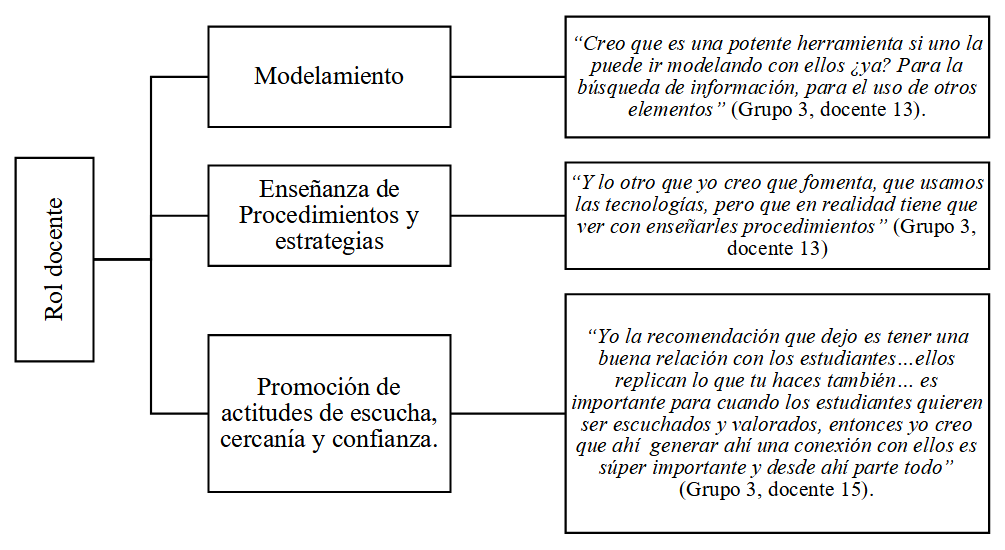
\includegraphics[width=0.8\textwidth]{fig33a.png}
 \caption{Rol docente desprendido del uso de App en contextos de aprendizaje virtual por pandemia.}
 \label{fig33a}
 %\source{Forneça aqui a fonte da imagem.}
\end{figure}

\begin{figure}[htbp]
 \centering
 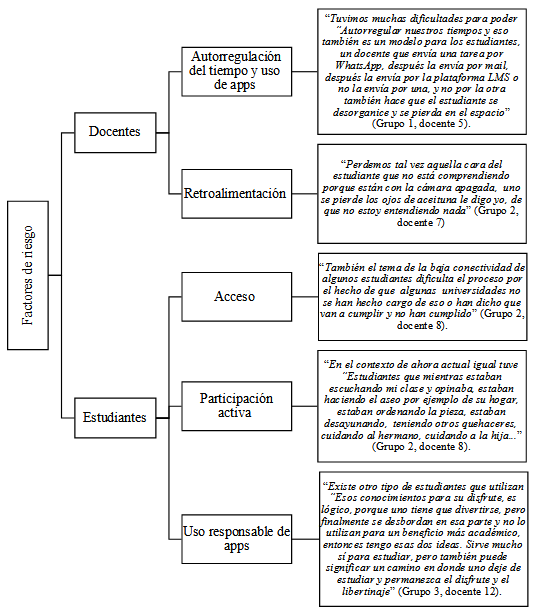
\includegraphics[width=0.65\textwidth]{fig33b.png}
 \caption{Factores de riesgo desprendidos del uso de App en contextos de aprendizaje virtual por pandemia.}
 \label{fig33b}
 %\source{Forneça aqui a fonte da imagem.}
\end{figure}

\begin{figure}[htbp]
 \centering
 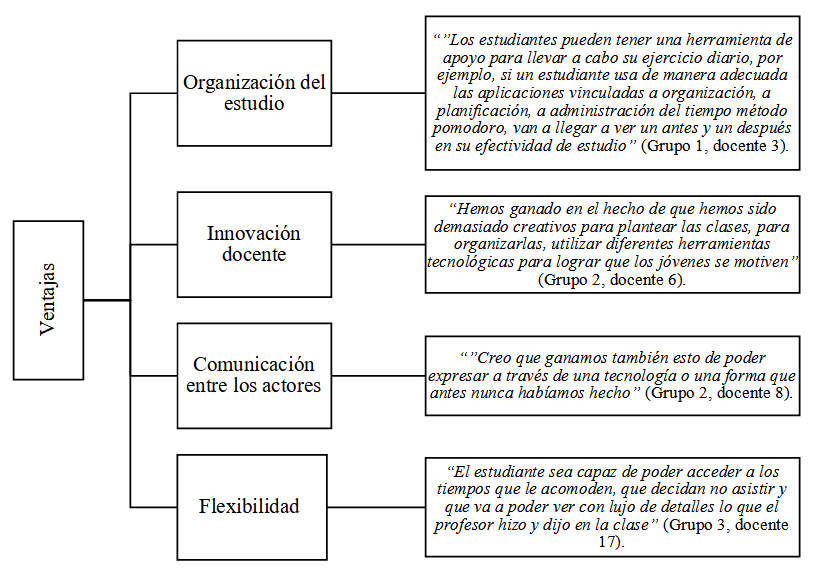
\includegraphics[width=0.8\textwidth]{fig33c.png}
 \caption{Ventajas desprendidas del empleo de App en contexto de enseñanza -aprendizaje virtual por pandemia.}
 \label{fig33c}
 %\source{Forneça aqui a fonte da imagem.}
\end{figure}

\section{Discusión}
En este estudio exploratorio de alcance descriptivo, se encontraron 34 App que el cuerpo docente participante utiliza en sus clases en modalidad virtual en contexto de pandemia por COVID-19. Es decir, la implementación del proceso de enseñanza-aprendizaje virtual por pandemia ha generado la necesidad de avanzar en el uso de aplicaciones digitales en la docencia universitaria. Además, la muestra de docentes usa diversas App para los procesos de enseñanza-aprendizaje en contexto de pandemia \cite{zamora-antunano2021, almarzooq2020, budianto2021, akaloo2021, pramana2021}. Para la autorregulación del aprendizaje el cuerpo docente reportó 27 App, las cuales en su mayoría resultan pertinentes para facilitar procesos de ejecución asociados a la fase 1, de acuerdo al modelo de \textcite[p. 142]{zimmerman2013}.

La App más utilizada por el profesorado para interactuar con sus estudiantes es WhatsApp; esta corresponde a una App que forma parte del grupo de aquellas que tienen fines distintos a los educativos, sin embargo esta investigación reveló que ha sido la más usada con fines de aprendizaje en línea por parte de la muestra de docentes durante este tiempo de pandemia por COVID-19. Al parecer, la preferencia con esta App se relaciona con la accesibilidad en términos de consumo de datos y la cercanía docente-estudiante que facilita la instantaneidad de la App. Estudios anteriores refieren que WhatsApp es un sistema con una interfaz simple,  coherente y visualmente autodescriptiva. Es considerada como una App de fácil uso debido a su eficiencia y fácil aprendizaje, además del bajo costo \cite{correia2020}. Del mismo modo ha demostrado tener impacto positivo en los procesos de aprendizaje del estudiantado, utilizando esta aplicación como un recurso de apoyo para compartir materiales multimedias pequeños y como un canal de comunicación entre el profesor-alumno fuera del horario de clases (So, 2016), sin embargo, en comparación con Zoom, Skype y Teams, WhatsApp es inferior a la hora de crear y respaldar la enseñanza y el aprendizaje en línea, por tanto puede ser adecuado sólo para discusiones en grupos pequeños y conferencias a pequeña escala \cite{correia2020}. En este sentido, sería interesante explorar cómo es la percepción de apoyo del estudiante y como las limitaciones de esta App genera sobrecarga en la labor del docente.

WhatsApp y Google Calendar son las App más recomendadas por el profesorado. En el caso del Google Calendar, este es parte de los servicios de Google App, que han sido empleados para la educación, esta aplicación permite organizar las actividades productivas de profesores y estudiantes en conjunto, permitiendo fomentar de manera remota la organización del tiempo para el desarrollo de las actividades académicas. Otros estudios refieren el potencial de esta App para la gestión y presentación de horarios de clases, consultas, exámenes; horarios de servicio; calendarios de observaciones, conferencias, olimpiadas, proyectos, exposiciones, fechas significativas, entre otros eventos, propiciando de esta forma la motivación y la participación activa del estudiante a las actividades académicas \cite{samerkhanova_developing_2017, amiruddin2020}. En función de los hallazgos encontrados y de la información provista en la evidencia científica, estas aplicaciones, en términos de la promoción de la autorregulación del aprendizaje en  estudiantes, podrían estar relacionadas más con la fase de preparación. Especial valor  le otorga el profesorado a la generación de vínculos positivos con los  estudiantes, basados en la empatía y valoración, constituyendo los cimientos sobre los cuales se co-construye el proceso de enseñanza-aprendizaje, adquiriendo mayor  importancia en contextos virtuales de aprendizaje por pandemia, puesto que contribuye a desarrollo de actitudes de pertenencia \cite{macfarlane2018}. 

Un aspecto interesante de resaltar  destacar es que, aun cuando las App antes descritas no han sido diseñadas para la promoción de la autorregulación y  por sí mismas no promueven estas conductas en estudiantes, en coherencia con el testimonio compartido en los grupos focales, pueden ser potencialmente apropiadas para fomentar estas estrategias en los  estudiantes, en un proceso que implica la participación activa del docente, en la forma en cómo  se diseñan las tareas académicas e intencionan las estrategias didácticas durante la experiencia educativa \cite{valencia2017, weepiu2020, martinez-sarmiento2018, castro2016}.

Las relatorías grupales muestran que las App preferentemente empleadas en la enseñanza universitaria en modalidad virtual en tiempos de pandemia, corresponden a App híbridas, seguidas por las  App nativas y finalmente las App basadas en la web \cite[p. 12-13]{santiago_mobile_2015}. El uso de App híbridas permite o garantiza que las aplicaciones sean más efectivas cuando el estudiante se planifica independientemente del dispositivo que utilice (teléfono celular o computador), recibe recordatorios o realiza otras actividades en las cuales la App permite sincronizar  avisos de gran valor para la realización de las actividades académicas. En este sentido, la experiencia docente en uso de App en pandemia se caracteriza por ser  diversa y flexible, puesto que  no sólo incluye el uso de App educativas sino que también y  en mayor medida, aquellas que en principio estarían diseñadas para propósitos laborales  y finalmente App que facilitan la organización en distintos contextos. 

Un resultado relevante de este estudio son las implicancias del uso de App, que se pueden inferir a partir de los relatos grupales, específicamente  en relación a un conjunto de factores de riesgo en la enseñanza virtual, las   ventajas  de las App para favorecer aprendizaje autorregulado y los desafíos asociados al rol del/a docente universitario/a en contexto de educación remota por  pandemia. A partir de las dificultades experimentadas por la muestra de participantes en esta investigación, es posible señalar que la docencia tiene el desafío de generar autorreflexión para el uso consciente de App para los procesos autorregulatorios y retroalimentar \cite[p. 272]{valencia-serrano2020} en este contexto de virtualidad, siendo  necesario que el cuerpo docente tenga la experiencia de una retroalimentación efectiva, aprovechando al máximo las ventajas y atenuando las brechas de la virtualidad \cite[p. 54]{instituto_internacional_para_la_educacion_superior_en_america_latina_y_el_caribe_covid-19_2020},  para  brindar una retroalimentación  oportuna, precisa y propositiva, que valore el esfuerzo y los intentos de los  estudiantes por mejorar \cite[p. 74]{dapelo2021}, contribuyendo de este modo al sentido de pertenencia \cite{masika2016}. 

Respecto a las experiencias compartidas por los grupos en relación a la docencia virtual en tiempos de pandemia, es posible reconocer algunas prácticas docentes que potenciarán la autonomía en los estudiantes  tales como (1) modular las App para favorecer el procesamiento de la información, (2) crear oportunidades de aprendizaje estratégico, (3) escuchar con atención, (4) promover la cercanía, valoración y confianza, (5) proporcionar oportunidades para que el estudiantado se exprese y (6) innovar para provocar la motivación en los  estudiantes. En este sentido, estas prácticas encierran un conjunto de competencias que trascienden a las propiamente disciplinares,  tradicionalmente muy valoradas  en educación superior, y que de una y otra forma, el cambio abrupto desde una educación presencial a una  virtual  por  emergencia sanitaria, puso  sobre la mesa, interpelando a todos los/as actores a revisar sus creencias, conocimientos y valores en torno al sentido de la docencia en tiempos de alta complejidad y en un escenario poco familiar. Así, reconociendo las ventajas y bondades del uso de las App, se levanta la necesidad de fortalecer el acompañamiento docente en los procesos de autorregulación mediados por tecnología en contexto de pandemia \cite{diazmujica2017, ninocarrasco2019}.

Las lecciones aprendidas, a partir de las experiencias de enseñanza virtual de la muestra de participantes en pandemia por  COVID-19, sin lugar a dudas que  invitan a reflexionar en torno a la responsabilidad social de las instituciones de educación superior,  en  incorporar los avances tecnológicos para generar estructuras de oportunidades de aprendizaje  de calidad; accesibles, diversificadas y flexibles, para sus docentes y estudiantes, de modo de avanzar hacia un uso estratégico de las tecnologías, que contribuya efectivamente a fortalecer  el  rol social de la educación superior, en un escenario de alta complejidad a nivel global, caracterizado por el cambio,  la  incertidumbre y la innovación.

En este estudio se ha aportado conocimiento en torno al empleo de las aplicaciones digitales en la educación superior chilena, en contexto de pandemia por  COVID-19 y  se han identificado desafíos compartidos para avanzar hacia un  uso  progresivamente estratégico, que promueva la generación  de escenarios de aprendizajes mediados por la tecnología, inclusivos, equitativos y de  calidad \cite{instituto_internacional_para_la_educacion_superior_en_america_latina_y_el_caribe_covid-19_2020}.

\section{Conclusiones}
\begin{enumerate}
    \item El conocimiento sobre autorregulación del aprendizaje, uso y recomendación de aplicaciones digitales por parte de docentes comprenden aspectos relevantes en contexto de pandemia, ya que estos representan una oportunidad para la mejora de la calidad de los aprendizajes y para la renovación de metodologías para los procesos de autorregulación \cite[p. 69]{zimmerman2002}. 
    \item Las  relatorías del cuerpo docente permiten apreciar el empleo de  variadas aplicaciones en  la enseñanza virtual en contexto de pandemia, 34 App fueron identificadas; las cuales 27  pueden  aportar al fomento de la autorregulación del aprendizaje. 
    \item El uso de App tiende a potenciar de modo preferente procesos cognitivos y motivacionales relativos a la fase de preparación y menos para las fases de ejecución y de autorreflexión.
    \item Las bondades de  acceso y  uso de WhatsApp la han transformado en la App más utilizada para la docencia virtual en contexto de pandemia 
    \item La muestra de docentes reconoce implicancias del uso de App. Fueron identificados cinco factores de riesgo, los cuales se vieron reflejados tanto en dificultades docentes, relacionadas con la autorregulación del tiempo, uso de App y retroalimentación personal, precisa y constructiva, como en dificultades del estudiantado relacionadas con el acceso, la participación activa y el uso responsable de App. Respecto a las ventajas del uso de App, desde la perspectiva del profesorado, estas  favorecen la organización del estudio, la innovación docente, la comunicación y la flexibilidad. Finalmente, en cuanto al rol docente en un entorno virtual, se espera que cuente con los conocimientos que le permitan hacer un mejor uso y modelar el empleo de las App en sus estudiantes , para favorecer  así el procesamiento estratégico, fomentar la enseñanza de procedimientos / estrategias y promover  actitudes de escucha, cercanía y confianza en sus estudiantes, por medio de  tecnologías digitales accesibles y preparación apropiada, responsabilidad compartida por las instituciones formadoras,
\end{enumerate}

\section*{Agencia de Financiamiento}
Proyecto ANID-COVID1012: Desarrollo e implementación de procedimientos docentes para facilitar la disposición al aprendizaje en condiciones de distanciamiento físico por pandemia de la COVID-19, en asignaturas de primer año universitario con mediano o alto riesgo de fracaso.

Comisión Nacional de Investigación Científica y Tecnológica, Chile. CONICYT/Doctorado Nacional/Beca número 21202382.

\printbibliography\label{sec-bib}
% if the text is not in Portuguese, it might be necessary to use the code below instead to print the correct ABNT abbreviations [s.n.], [s.l.] 
%\begin{portuguese}
%\printbibliography[title={Bibliography}]
%\end{portuguese}

%full list: conceptualization,datacuration,formalanalysis,funding,investigation,methodology,projadm,resources,software,supervision,validation,visualization,writing,review
\begin{contributors}[sec-contributors]
\authorcontribution{Valeria Aylín Infante-Villagrán}[conceptualization,investigation,projadm,supervision,writing]
\authorcontribution{Bianca Maria Pia Dapelo Pellerano}[conceptualization,investigation,methodology,writing,review]
\authorcontribution{Rubia Cobo-Rendon}[conceptualization,investigation,writing,review]
\authorcontribution{Yaranay López-Angulo}[conceptualization,methodology,writing]
\authorcontribution{Bertha Escobar Alaniz}[review]
\authorcontribution{Christian Beyle}[conceptualization,datacuration,investigation,methodology,visualization,writing]
\end{contributors}


%\begin{contributors}{sec-contributors}
%\item \textbf{Valeria Aylín Infante-Villagrán}: Conceptualización; Investigación; Administración de proyecto; Supervisión; Redacción de borrador original
%\item \textbf{Bianca Maria Pia Dapelo Pellerano}: Conceptualización; Investigación; Metodología; Escritura; Redacción del borrador original; Redacción, revisión y edición
%\item \textbf{Rubia Cobo-Rendon}: Conceptualización; Investigación; Redacción del borrador original; Redacción, revisión y edición
%\item \textbf{Yaranay López-Angulo}: Conceptualización; Metodología; Redacción de borrador original
%\item \textbf{Bertha Escobar Alaniz}: Redacción, revisión y edición
%\item \textbf{Christian Beyle}: Conceptualización; Análsis de datos; Investigación; Metodología; Visualización; Redacción
%\end{contributors}

\end{document}
